\section{Aufbau der Evaluation}
Um die Hypothese zu beweisen oder zu widerlegen, werden [Anzahl] von angehenden und ausgebildeten Designern befragt. Für die Befragung wird den Probanden drei verschiedene Szenarien gezeigt, welche ungefähr die drei Szenarien aus Kapitel \ref{sec:szenarien} abbilden.

Den Probanden werden in einem flowws-Prototyp drei fertige Graphen gezeigt, die mit den drei Szenarien korrespondieren. Ziel der Endnutzer ist es, die verschiedenen Komponenten des Graphen zu identifizieren, ihre Funktion zu deuten und Rückschlüsse über ihr Verhalten zu ziehen. Wenn die Probanden das Verhalten des Graphen antizipieren können, wird im Dialog elaboriert, ob das mentale Modell, dass der Endnutzer gebildet hat, mit dem Konzeptmodell von flowws übereinstimmt. Wenn der Endnutzer das Verhalten des Graphen nicht antizipieren kann, werden im Dialog die Diskrepanzen zwischen dem Konzept- und dem mentalen Modell erörtert.

Der \textbf{Aufbau} und \textbf{Ablauf} der Evaluation ist wie folgt:
\begin{enumerate}
    \item Der Proband gibt Angaben zu seinen Merkmalen und schätzt sein Fachwissen hinsichtlich \ac{IoT}-Domäne und Programmierung ab (siehe Kapitel \ref{subsec:fragebogen}).
    \item Der Proband ließt zusammen mit dem Gutachter den Interview Leitfaden (siehe Kapitel \ref{subsec:leitfaden}) durch. Eventuelle Unklarheiten werden hierbei beseitigt. 
    \item Dem Proband werden nacheinander drei Graphen gezeigt. Nach jedem Graphen wird anhand eines Fragebogens geprüft, ob der Nutzer die Funktionen der einzelnen Komponenten sowie deren Zusammenspiel deuten kann. Es wird als Erfolg gesehen, wenn der Proband von selbst das abgebildete Szenario beschreiben kann, d.h. er hat verstanden, das eine LED von rot zu gelb zu grün wechselt und somit eine Ampel abbildet. 
    \item Nachdem alle drei Graphen abgearbeitet worden sind, werden generelle Fragen zum Konzeptmodell gestellt. Hierbei werden Fragen verwendet, die sich an den \textit{Cognitive Dimensions} nach \cite{blackwell2000cognitive} orientieren. Ziel ist es dabei grundsätzliche Schwächen, Stärken sowie Verbesserungspotential zu identifizieren.
\end{enumerate}

Um ein grundlegendes Verständnis für das Konzeptmodell zu erreichen bzw. dieses zu überprüfen, ist es nicht nötig, dass der Benutzer selbst den Graphen erstellt. Aus diesem Grund wird sich bei der Evaluation darauf beschränkt, den Nutzer bestehende Graphen zu analysieren zu lassen.

\subsection{Prototyp}

\begin{figure}[h]
  \centering
  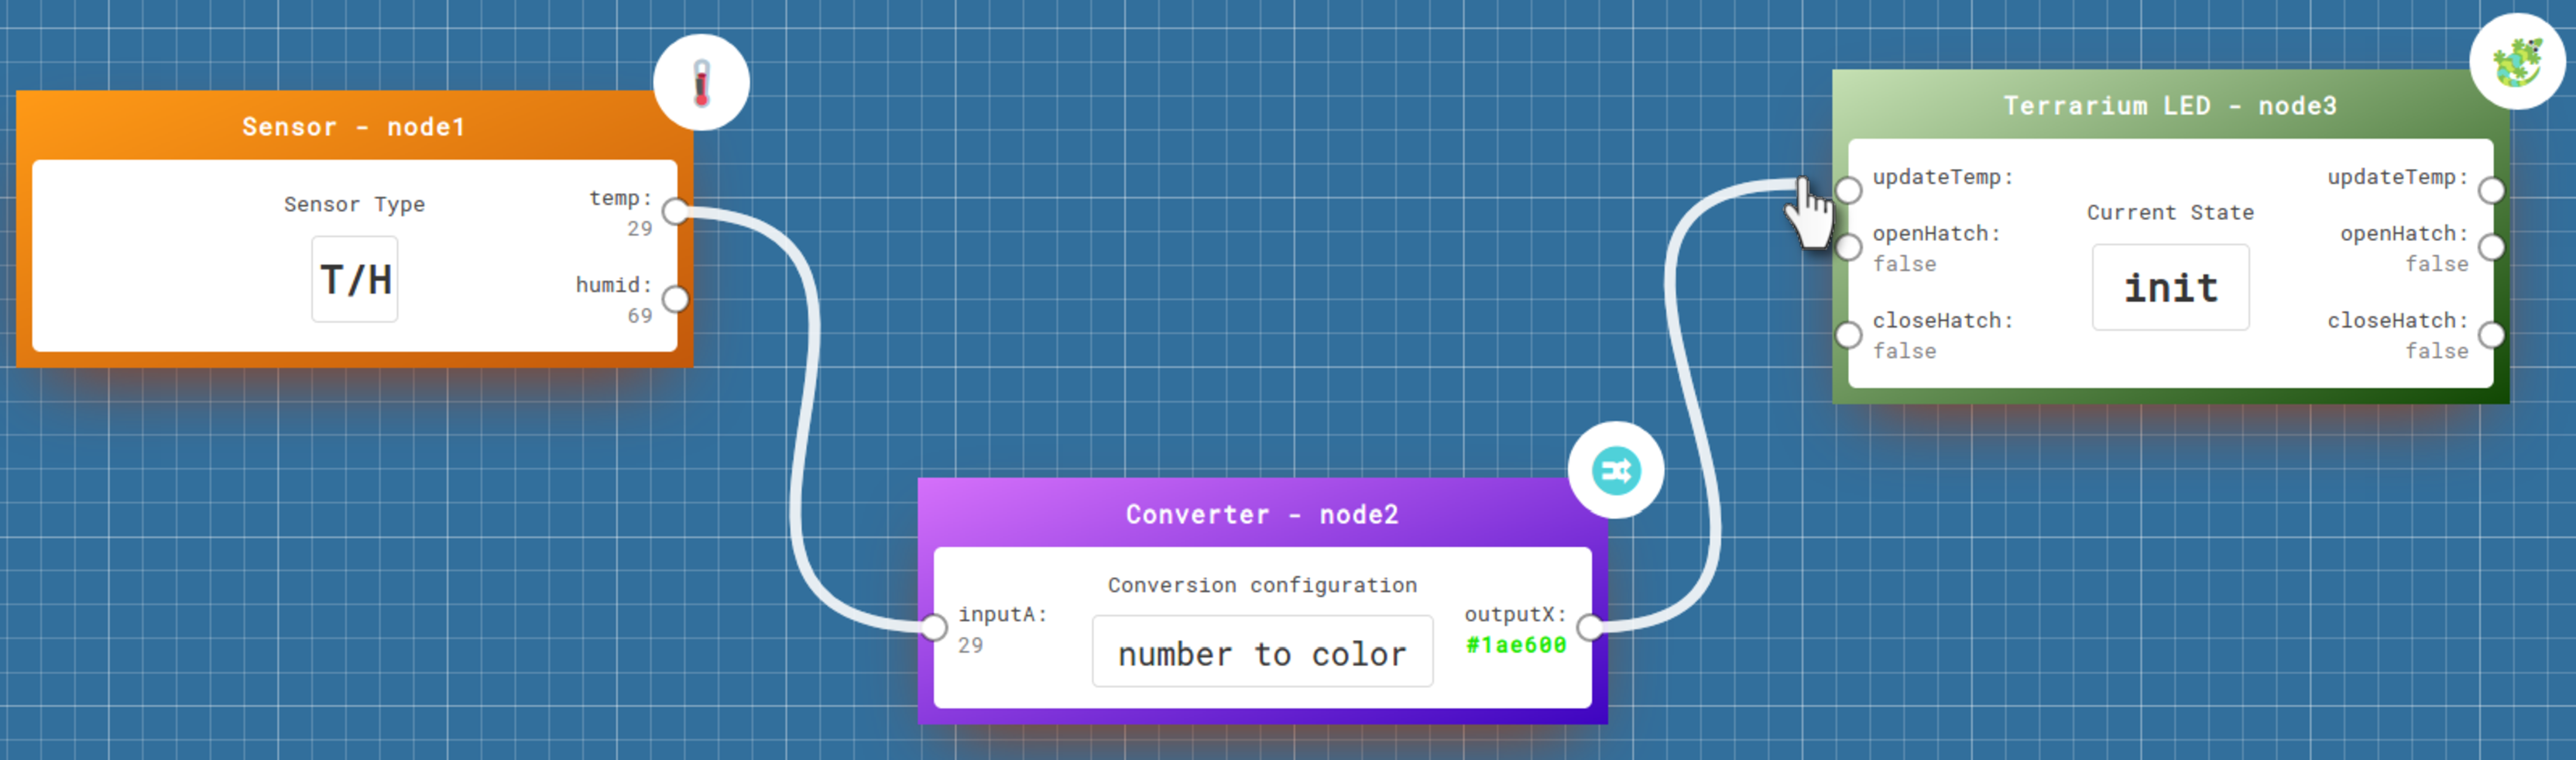
\includegraphics[width=1\textwidth]{bilder/chapter5/screenshotflows.pdf}
  \caption{Screenshot des flowws-Prototyps}
  \label{fig:genericnode}
\end{figure}

Für die Evaluation wurde im Zuge dieser Thesis eine prototypische Implementation von flowws erstellt. Der Prototyp kann die grundlegenden Elemente (Sensor-, Aktor- und Funktionsknoten, Verbindungen) von flowws darstellen und animieren. Darüber hinaus, lassen sich die Elemente miteinander kombinieren und die Signalverarbeitung des Graphen simulieren.

Der Sourcecode wurde als \textit{Webapp} mit dem React-Framework\footnote{\url{https://reactjs.org/} - besucht September 2018} erstellt und steht in einem \textit{Github-Repository}\footnote{\url{https://github.com/chrbrt/flowws} - besucht September 2018} zur freien Verfügung.